\begin{figure}[htbp]
    \centering
    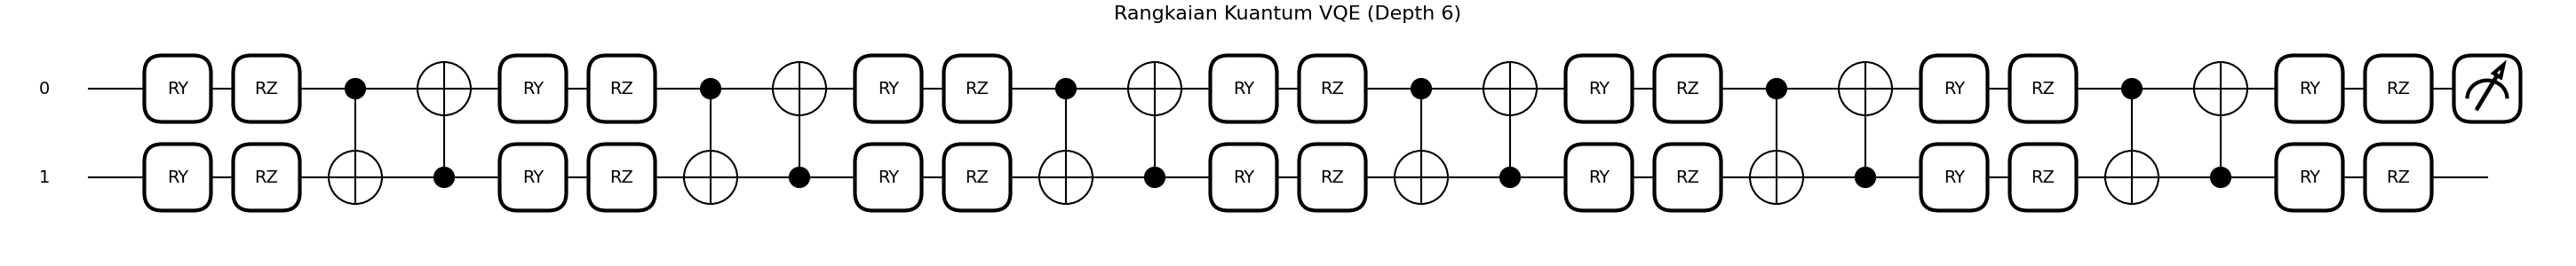
\includegraphics[width=\textwidth]{rangkaian_kuantum_depth6_N2.png}
    \caption{Representasi sirkuit kuantum variasional dengan struktur \textit{ansatz} yang terdiri dari operator $\hat{U}_A$, $\hat{U}(\theta)$, dan $\hat{U}_B$ untuk optimasi parameter $\theta$.}
    \label{fig:circuit_vqe}
\end{figure}

Untuk kasus 1 depth (8 parameter $\theta$):

\begin{equation}
    | \psi(\theta) \rangle = \hat{U}_{rot}^{(1)} (\theta_1) \cdot \hat{U}_{\hatent} \cdot \hat{U}_{rot}^{(0)} (\theta_0) |00\rangle
\end{equation}
dimana operator rotasi qubit $j$ layer $l$ didefinisikan sebagai $\hat{U}_{l,j} = R_z(\theta_{l,j,z}) R_y(\theta_{l,j,y})$ dengan representasi matriks:
\begin{equation}
    \hat{U}_{l,j} = \begin{pmatrix} e^{-i\frac{\theta_{l,j,z}}{2}} \cos\frac{\theta_{l,j,y}}{2} & -e^{-i\frac{\theta_{l,j,z}}{2}} \sin\frac{\theta_{l,j,y}}{2} \\ e^{i\frac{\theta_{l,j,z}}{2}} \sin\frac{\theta_{l,j,y}}{2} & e^{i\frac{\theta_{l,j,z}}{2}} \cos\frac{\theta_{l,j,y}}{2} \end{pmatrix}
\end{equation}
dan $\hat{U}_{rot}^{(l)} = \hat{U}_{l,0} \otimes \hat{U}_{l,1}$. Operator entrainment $\hat{U}_{ent}$ merupakan cascade CNOT:
\begin{equation}
    \hat{U}_{ent} = CNOT_{q_1, q_0} \cdot CNOT_{q_0,q_1} = \begin{pmatrix} 1 & 0 & 0 & 0 \\ 0 & 0 & 1 & 0 \\ 0 & 0 & 0 & 1 \\ 0 & 1 & 0 & 0 \end{pmatrix}
\end{equation}
Penurunan state dilakukan secara sekuensial. Aplikasi rotasi pertama pada $|00\rangle$ menghasilkan:
\begin{equation}
    |\phi_0\rangle = \hat{U}_{rot}^{(0)}|00\rangle = \begin{pmatrix} e^{-i\frac{\theta_{0,0,z}+\theta_{0,1,z}}{2}} \cos\frac{\theta_{0,0,y}}{2} \cos\frac{\theta_{0,1,y}}{2} \\ e^{-i\frac{\theta_{0,0,z}-\theta_{0,1,z}}{2}} \cos\frac{\theta_{0,0,y}}{2} \sin\frac{\theta_{0,1,y}}{2} \\ e^{i\frac{\theta_{0,0,z}-\theta_{0,1,z}}{2}} \sin\frac{\theta_{0,0,y}}{2} \cos\frac{\theta_{0,1,y}}{2} \\ e^{i\frac{\theta_{0,0,z}+\theta_{0,1,z}}{2}} \sin\frac{\theta_{0,0,y}}{2} \sin\frac{\theta_{0,1,y}}{2} \end{pmatrix}
\end{equation}
Aplikasi operator entrainment $\hat{U}_{ent}$ pada $|\phi_0\rangle$ menghasilkan $|\phi_1\rangle$:
\begin{equation}
    |\phi_1\rangle = \hat{U}_{ent}|\phi_0\rangle = \begin{pmatrix} e^{-i\frac{\theta_{0,0,z}+\theta_{0,1,z}}{2}} \cos\frac{\theta_{0,0,y}}{2} \cos\frac{\theta_{0,1,y}}{2} \\ e^{i\frac{\theta_{0,0,z}-\theta_{0,1,z}}{2}} \sin\frac{\theta_{0,0,y}}{2} \cos\frac{\theta_{0,1,y}}{2} \\ e^{i\frac{\theta_{0,0,z}+\theta_{0,1,z}}{2}} \sin\frac{\theta_{0,0,y}}{2} \sin\frac{\theta_{0,1,y}}{2} \\ e^{-i\frac{\theta_{0,0,z}-\theta_{0,1,z}}{2}} \cos\frac{\theta_{0,0,y}}{2} \sin\frac{\theta_{0,1,y}}{2} \end{pmatrix}
\end{equation}
State akhir $|\psi(\theta)\rangle$ diperoleh dengan mengaplikasikan rotasi layer kedua:
\begin{equation}
    |\psi(\theta)\rangle = \hat{U}_{rot}^{(1)}|\phi_1\rangle = (\hat{U}_{1,0} \otimes \hat{U}_{1,1}) |\phi_1\rangle
\end{equation}
\begin{equation}
    \hat{U}(\theta) = \mathbb{I} \otimes \hat{R}_y(\theta) = 
    \begin{pmatrix} 
    \cos\frac{\theta}{2} & -\sin\frac{\theta}{2} & 0 & 0 \\ 
    \sin\frac{\theta}{2} & \cos\frac{\theta}{2} & 0 & 0 \\ 
    0 & 0 & \cos\frac{\theta}{2} & -\sin\frac{\theta}{2} \\ 
    0 & 0 & \sin\frac{\theta}{2} & \cos\frac{\theta}{2} 
    \end{pmatrix}
\end{equation}

\begin{equation}
    \hat{U}_B = \prod_{j=k+1}^{m} \hat{G}_j, \quad \hat{G}_j \in \mathbb{C}^{4 \times 4}
\end{equation}
dimana $\hat{G}_j$ merupakan operator unitari (gate) pada sirkuit post-processing.

\begin{equation}
    \hat{U}(\theta) = e^{-i \frac{\theta}{2} \hat{P}}
\end{equation}

\begin{equation}
    | \phi \rangle = \hat{U}_A | 0 \rangle
\end{equation}

\begin{equation}
    \hat{M} = \hat{U}_B^{\dagger} \hat{H} \hat{U}_B
\end{equation}

\begin{align}
    E(\theta) &= \langle \phi | \hat{U}^{\dagger}(\theta) \hat{M} \hat{U}(\theta) | \phi \rangle
\end{align}

\begin{equation}
    \frac{\partial \hat{U}(\theta)}{\partial \theta} = -i \frac{1}{2} \hat{P} \hat{U}(\theta)
\end{equation}

\begin{equation}
    \frac{\partial \hat{U}^{\dagger}(\theta)}{\partial \theta} = i \frac{1}{2} \hat{U}^{\dagger}(\theta) \hat{P}
\end{equation}

\begin{align}
    \frac{\partial E(\theta)}{\partial \theta} &= \langle \phi | \frac{\partial \hat{U}^{\dagger}(\theta)}{\partial \theta} \hat{M} \hat{U}(\theta) | \phi \rangle + \langle \phi | \hat{U}^{\dagger}(\theta) \hat{M} \frac{\partial \hat{U}(\theta)}{\partial \theta} | \phi \rangle \\
    \frac{\partial E(\theta)}{\partial \theta} &= \frac{i}{2} \langle \phi | \hat{U}^{\dagger}(\theta) \hat{P} \hat{M} \hat{U}(\theta) | \phi \rangle - \frac{i}{2} \langle \phi | \hat{U}^{\dagger}(\theta) \hat{M} \hat{P} \hat{U}(\theta) | \phi \rangle
\end{align}

\begin{equation}
    [\hat{P}, \hat{U}(\theta)] = 0 \implies \hat{P} \hat{U}(\theta) = \hat{U}(\theta) \hat{P}
\end{equation}

\begin{align}
    \frac{\partial E(\theta)}{\partial \theta} &= \frac{i}{2} \langle \phi | \hat{U}^{\dagger}(\theta) [\hat{P}, \hat{M}] \hat{U}(\theta) | \phi \rangle
\end{align}

\begin{equation}
    | \psi(\theta) \rangle = \hat{U}(\theta) | \phi \rangle
\end{equation}

\begin{equation}
    \frac{\partial E(\theta)}{\partial \theta} = \frac{i}{2} \langle \psi(\theta) | [\hat{P}, \hat{M}] | \psi(\theta) \rangle
\end{equation}

\begin{align}
    E(\theta + s) &= \langle \psi(\theta) | e^{i \frac{s}{2} \hat{P}} \hat{M} e^{-i \frac{s}{2} \hat{P}} | \psi(\theta) \rangle \\
    E(\theta + s) &= \langle \psi(\theta) | \left[ \cos^2\left(\frac{s}{2}\right) \hat{M} + i \sin\left(\frac{s}{2}\right)\cos\left(\frac{s}{2}\right) [\hat{P}, \hat{M}] + \sin^2\left(\frac{s}{2}\right) \hat{P} \hat{M} \hat{P} \right] | \psi(\theta) \rangle
\end{align}

\begin{align}
    E(\theta - s) &= \langle \psi(\theta) | e^{-i \frac{s}{2} \hat{P}} \hat{M} e^{i \frac{s}{2} \hat{P}} | \psi(\theta) \rangle \\
    E(\theta - s) &= \langle \psi(\theta) | \left[ \cos^2\left(\frac{s}{2}\right) \hat{M} - i \sin\left(\frac{s}{2}\right)\cos\left(\frac{s}{2}\right) [\hat{P}, \hat{M}] + \sin^2\left(\frac{s}{2}\right) \hat{P} \hat{M} \hat{P} \right] | \psi(\theta) \rangle
\end{align}

\begin{align}
    E(\theta + s) - E(\theta - s) &= 2i \sin\left(\frac{s}{2}\right)\cos\left(\frac{s}{2}\right) \langle \psi(\theta) | [\hat{P}, \hat{M}] | \psi(\theta) \rangle \\
    E(\theta + s) - E(\theta - s) &= i \sin(s) \langle \psi(\theta) | [\hat{P}, \hat{M}] | \psi(\theta) \rangle
\end{align}

\begin{equation}
    s = \frac{\pi}{2} \implies \sin\left(\frac{\pi}{2}\right) = 1
\end{equation}

\begin{equation}
    E\left(\theta + \frac{\pi}{2}\right) - E\left(\theta - \frac{\pi}{2}\right) = i \langle \psi(\theta) | [\hat{P}, \hat{M}] | \psi(\theta) \rangle
\end{equation}

\begin{align}
    \frac{\partial E(\theta)}{\partial \theta} &= \frac{1}{2} \left( i \langle \psi(\theta) | [\hat{P}, \hat{M}] | \psi(\theta) \rangle \right) \\
    \frac{\partial E(\theta)}{\partial \theta} &= \frac{1}{2} \left[ E\left(\theta + \frac{\pi}{2}\right) - E\left(\theta - \frac{\pi}{2}\right) \right]
\end{align}

\begin{equation}
    \theta_{n+1} = \theta_n - \eta \frac{\partial E(\theta_n)}{\partial \theta}
\end{equation}

\begin{equation}
    \theta^{(0)} = \frac{\pi}{4}, \quad s = \frac{\pi}{2}
\end{equation}

\begin{align}
    \theta_+ &= \theta^{(0)} + s = \frac{3\pi}{4} \\
    P(1)_+ &= \sin^2\left(\frac{3\pi}{8}\right) \approx 0.8535 \\
    E(\theta_+) &= 10(P(0)_+ - P(1)_+) = 10(0.1465 - 0.8535) = -7.07
\end{align}

\begin{align}
    \theta_- &= \theta^{(0)} - s = -\frac{\pi}{4} \\
    P(1)_- &= \sin^2\left(-\frac{\pi}{8}\right) \approx 0.1465 \\
    E(\theta_-) &= 10(P(0)_- - P(1)_-) = 10(0.8535 - 0.1465) = 7.07
\end{align}

\begin{align}
    \frac{\partial E(\theta^{(0)})}{\partial \theta} &= \frac{1}{2} (E(\theta_+) - E(\theta_-)) \\
    \frac{\partial E(\theta^{(0)})}{\partial \theta} &= \frac{1}{2} (-7.07 - 7.07) = -7.07
\end{align}

\begin{equation}
    \theta^{(1)} = \theta^{(0)} - \eta \frac{\partial E(\theta^{(0)})}{\partial \theta} = \frac{\pi}{4} + 7.07 \eta
\end{equation}
